\documentclass[12pt,fleqn]{article}\usepackage{../../common}
\begin{document}
Ders 17

Sınırlı Öğeler Metodu (Finite Elements Method)

Bu metot differansiyel, kısmı differansiyel denklemleri (partial
differential equations) yaklaşıksal olarak modelleme ve çözmenin
yöntemleridir.

Formül: Başlangıç denklemi

$$ \frac{-d}{\ud x} \bigg( c(x) \ \frac{\ud u}{\ud x} \bigg) = f(x) $$

İki tarafı da  $v(x)$ ile çarpıyoruz ve 0 to 1 sınırlarıyla entegralini alıyoruz.

$$
\int_0^1 \frac{-d}{\ud x} \bigg( c(x) \frac{\ud u}{\ud x} \bigg) v(x)\ud x
= \int_0^1 f(x)v(x) \ud x
$$

Parçalı entegral (integration by parts) formülü şöyledir:

$$ \int y \ud z = y  z - \int z \ud y $$

Ana formülün bölümlerini, parçalı entegrale göre bölüştürürsek:

$$ dz = \frac{-d}{dx} \bigg( c(x) \ \frac{du}{dx} \bigg) dx  $$

$$ z = - c(x) \ \frac{du}{dx}  $$

$$ y = v(x)  $$

$$ dy = \frac{dv}{dx}dx $$

Yukarıda $dz$ içinde $dx$ ve $\frac{1}{dx}$ birbirini iptal eder. Parçalı
entegral formülünün sağ tarafına göre yerlerine koyarsak:

$$
\int_0^1 v(x)\ud x \frac{-d}{\ud x} \bigg( c(x) \frac{\ud u}{\ud x} \bigg)
= - \bigg[ v(x) c(x) \frac{\ud u}{\ud x} \bigg]_{x=0}^{x=1} \int_0^1 c(x) \frac{\ud u}{\ud x} \frac{\ud v}{\ud x} \ud x
$$

Üstteki parçalı entegral açılımında sol taraf entegrale sınır
değerleri aldığında, sağ taraftaki $yz$ sonucunun aynı sınır
değerlerine tabi olduğuna dikkat edelim.

Differansiyel denklemde sınır koşulları $x=1$ durumunda $c(1)u'(1)=0$,
ve $x=0$ durumunda $v(0)=0$ olarak biliniyor. O zaman üstteki
denklemin sol tarafında $x=0$ ve $x=1$ koşulları için tanımlı bölüm $0
- 0 = 0$ olacaktır ve denklemden atılabilir. Geriye kalanlar

$$
\int_0^1 c(x) \frac{\ud u}{\ud x} \frac{\ud v}{\ud x} \ud x
= \int_0^1 f(x)v(x) \ud x
$$

Bu fonksiyonu Galerkin adlı bir matematikçi bulmuş, "zayıf form (weak
form)" olarak adlandırılıyor.

Şimdi diyelim ki n tane test fonksiyonu seçtik $\phi_1(x),..,\phi(n)$
ve bu fonksiyonların $U_j$ sayıları ile çarpımının toplamını, yani bir
tür kombinasyonunu $u(x)$ yerine kullanmaya karar verdik.

$$ U(x) = U_1 \phi_1+ ... + U_n\phi_n $$

O zaman

$$ U'(x) = U_1 \phi_1'+ ... + U_n\phi_n' $$

$$ = \sum_1^n U_j \frac{d\phi_j}{dx} $$

Şimdi $du / dx$ yerine $U'(x)$ koyarsak

$$
\int_0^1 c(x) \bigg( \sum_1^n U_j \frac{\ud\phi_j}{\ud x}\bigg)
\frac{\ud V_i}{\ud x}\ud x
= \int_0^1 f(x)V_i(x)\ud x
$$

Dikkat edelim, $v(x)$ yerine $V_i(x)$ kullandık. Üstteki formül her i için yeni
bir formül "üretecek". Niye $V_i$? Zayıf formdaki $v(x)$ formülünü de zaten
biz uydurmuştuk, yani $v(x)$ biz ne istersek o olur. O zaman bu fonksiyonu n
tane formül üretmek için bir numara olarak kullanılıyoruz, n tane formül olunca
matrisin n x n elemanını doldurabileceğiz ve çözüme erişebileceğiz. Ek not,
çoğunlukla $V_i(x)$ için $\phi_i$ formülleri kullanılıyor. 

Ayrıca formüldeki $U_j$ kısmını cekip çıkartırsak ve bir vektör içine koyarsak,
geri kalanlar bir $K_{ij}$ matrisi içinde tutulabilir. 

$$ K_{ij} = \int_0^1 c(x) \frac{\ud\phi_j}{\ud x} \frac{\ud V_i}{\ud x} \ud x  $$

Sağ taraf aynı şekilde i tane formül üretir

$$ F_i = \int_0^1 f(x)V_i(x) \ud x $$

Final formül matrix formunda basit bir şekilde temsil edilebilecektir. 

$$ KU = F $$

Örnek

Örnek olarak $-u'' = 1$ denklemini çözelim. Not: Differansiyel
denklemlerde sonuç bulmak demek bir "fonksiyon" bulmak
demektir. Normal cebirsel denklemlerde sonuç bulmak değişkenlerin
"sayısal" değerini bulmak demektir. Birazdan bulacağımız sonuç
$u(x)$ "fonksiyonu" olacak.

Eğer denklem $-u''=1$ ise o zaman bu formülü ana forma uygun hale
getirmek için $c(x) = 1$ olarak almamız gerekir. $-u''=1$ denkleminde
eşitliğin sağ tarafı 1 olduğuna göre $f(x) = 1$ demektir.

Artık $\phi$ fonksiyonlarını seçme zamanı geldi. Bu fonksiyonların
"toplamı" hedeflediğimiz fonksiyonu yaklaşıksal (approximate) olarak
temsil edecek. Örnek olarak seçebileceğimiz bir fonksiyon "şapka
fonksiyonu (hat function)" olarak bilinen üçgen fonksiyonlar
olabilir. Alttaki figürde bu fonksiyonları görüyoruz.

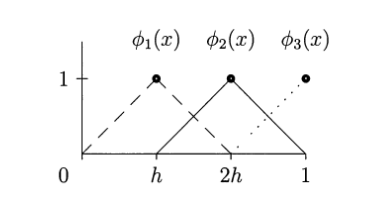
\includegraphics[height=4cm]{fem_hat.png}

Bu figürde x ekseninin h büyüklüğündeki parçalara bölündüğünü görüyoruz. 

Entegralleri hesaplayalım

$$ F_1 = \int_0^1 V_1(x) \ud x $$

Daha önce $V_1$ ve $\phi_1$'i aynı kabul ettiğimizi belirtmiştik. 

Yukarıdaki entegralin aslında bir alan hesabı yaptığını
görüyoruz. Sınırlar $0$ ve $1$ arasında, ama $2h$ ötesinde zaten
$\phi_1$ fonksiyonu yok. $\phi_1$'in alanı nedir? Alan üçgenin alanı:
Taban çarpı yükseklik bölü 2: $2h$, yüksekliği $1$, o zaman alan $(2h
\times 1) / 2 = 1/3$

Benzer mantıkla bakarsak, $F_2$ ile $F_1$ aynı, yani $1/3$. $F_3$ ise
onların yarısı, yani $1/6$.

$K_{ij}$ nasıl hesaplanacak? $c(x) = 1$ olduğu için formülden
çıkarılabilir ve $V_1$ ve $\phi_1$'in aynı olduğuna söyledik:

$$ K_{ij} = \int_0^1 c(x) \frac{\ud\phi_j}{\ud x} \frac{\ud V_i}{\ud x} \ud x $$

$$ K_{11} = \int_0^1 \bigg( \frac{\ud V_1}{\ud x} \bigg) ^2 \ud x  $$

$dV_1/dx$ nedir? Birinci şapka fonksiyonunun türevidir. Bu türeve
bakarsak, $0$ ve $h$ arasında artı eğim (slope) $1/h$, $h$ ve $2h$
arasında eksi eğim $-1/h$ oluyor. Ama kare aldığımız için sonuç aynı,
$1/h^2$. O zaman h = 1/3 olduğuna göre $1/(1/3)^2$, yani $dV_1/dx =
9$.

$$ K_{11} = \int_0^{2/3} 9 \ud x = 9x \bigg|_0^{2/3} = (9)(2/3) - 0 = 6 $$

$K_{22}$ şeklen aynı fonksiyon parçasını temel aldığı için aynı değere
sahip: 6. $K_{33}$ onların yarısı, eşittir 3.

$K_{12}$ farklı eğimlerin çarpımı anlamına gelir, yani $V_1'$ ile
$V_2'$ çarpımı olur. Bu iki fonksiyona bakalım, 0 ile h arasında $V_2$
yok, eğim 0. İkisinin de sıfır olmadığı, çarpımda kullanılabilecek bir
eğiminin olduğu tek aralık h ve 2h arası. Burada $V_1' = -3, V_2 = 3$.

$$
K_{12} = \int_{1/3}^{2/3} (3)(-3) \ud x
= -9x \bigg|_{1/3}^{2/3} = -6 - (-3) = -3
$$

Aynı şekilde $K_{23} = -3$. Ama $K_{13} = 0$ çünkü hiç çakışma yok.

Matrisi doldurursak, 

$$
KU = F
$$

$$ 
\left[\begin{array}{ccc}
    6 & -3 & 0 \\
    -3 & 6 & -3 \\
    0 & -3 & 3     
\end{array}\right]
\left[\begin{array}{c}
    U_1 \\
    U_2 \\
    U_3
\end{array}\right]
=
\left[\begin{array}{c}
    1/3 \\
    1/3 \\
    1/6
\end{array}\right]
$$

Python kodu 

\begin{minted}[fontsize=\footnotesize]{python}
K = [[6., -3., 0],
     [-3., 6., -3.],
     [0., -3., 3.]]

f = [1./3., 1./3., 1./6.]

print np.linalg.solve(K,f)
\end{minted}

\begin{verbatim}
[ 0.27777778  0.44444444  0.5       ]
\end{verbatim}

\begin{minted}[fontsize=\footnotesize]{python}
print 5./18., 4./9., 1./2.
\end{minted}

\begin{verbatim}
0.277777777778 0.444444444444 0.5
\end{verbatim}

Rapor edilen değerler bu denklemin bilinen çözümü $u(x) = x - \frac{1}{2}x^2$ 
ile 0, h, 2h noktalarında (mesh points) birebir uyum gösterdiğini
görüyoruz.  Yani yaklaşıksal olarak differansiyel denklemi çözmeyi 
başardık.

Kaynaklar

[1] Strang, G., {\em Computational Science and Engineering}




\end{document}
